\documentclass{article}
\usepackage{tikz}

\begin{document}

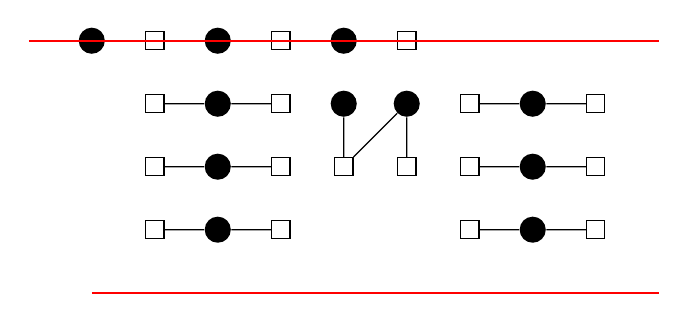
\begin{tikzpicture}[scale=0.8]
    % Define coordinates for nodes
    \node (A) at (0,0) [circle, fill=black] {};
    \node (B) at (1,0) [rectangle, draw] {};
    \node (C) at (2,0) [circle, fill=black] {};
    \node (D) at (3,0) [rectangle, draw] {};
    \node (E) at (4,0) [circle, fill=black] {};
    \node (F) at (5,0) [rectangle, draw] {};
    
    \node (G) at (1,-1) [rectangle, draw] {};
    \node (H) at (2,-1) [circle, fill=black] {};
    \node (I) at (3,-1) [rectangle, draw] {};
    
    \node (J) at (1,-2) [rectangle, draw] {};
    \node (K) at (2,-2) [circle, fill=black] {};
    \node (L) at (3,-2) [rectangle, draw] {};
    
    \node (M) at (1,-3) [rectangle, draw] {};
    \node (N) at (2,-3) [circle, fill=black] {};
    \node (O) at (3,-3) [rectangle, draw] {};
    
    \node (P) at (4,-1) [circle, fill=black] {};
    \node (Q) at (4,-2) [rectangle, draw] {};
    \node (R) at (5,-1) [circle, fill=black] {};
    \node (S) at (5,-2) [rectangle, draw] {};
    
    \node (T) at (6,-1) [rectangle, draw] {};
    \node (U) at (7,-1) [circle, fill=black] {};
    \node (V) at (8,-1) [rectangle, draw] {};
    
    \node (W) at (6,-2) [rectangle, draw] {};
    \node (X) at (7,-2) [circle, fill=black] {};
    \node (Y) at (8,-2) [rectangle, draw] {};
    
    \node (Z) at (6,-3) [rectangle, draw] {};
    \node (AA) at (7,-3) [circle, fill=black] {};
    \node (BB) at (8,-3) [rectangle, draw] {};
    
    % Draw edges
    \draw (A) -- (B);
    \draw (B) -- (C);
    \draw (C) -- (D);
    \draw (D) -- (E);
    \draw (E) -- (F);
    
    \draw (G) -- (H);
    \draw (H) -- (I);
    
    \draw (J) -- (K);
    \draw (K) -- (L);
    
    \draw (M) -- (N);
    \draw (N) -- (O);
    
    \draw (P) -- (Q);
    \draw (Q) -- (R);
    \draw (R) -- (S);
    
    \draw (T) -- (U);
    \draw (U) -- (V);
    
    \draw (W) -- (X);
    \draw (X) -- (Y);
    
    \draw (Z) -- (AA);
    \draw (AA) -- (BB);
    
    % Draw red lines
    \draw[red, thick] (-1,0) -- (9,0);
    \draw[red, thick] (0,-4) -- (9,-4);
\end{tikzpicture}

\end{document}